\chapter{Conclusion And Future Work}
\section{Conclusion}
This research shows how Vose's haploid model for Genetic Algorithms
extends to the diploid case, facilitating the computation of infinite
population evolutionary trajectories by significantly reducing the
time and space used.  Efficiency is achieved through reducing diploid evolution 
to the evolution of haploid populations
and employing Walsh transform methods to compute the effects of
mask-based crossover and mutation.  

Simulations are thereby made feasible which otherwise would require
excessive resources, as illustrated through computations exploring 
the convergence rate of finite population short-term behavior to infinite population evolutionary trajectories. 
Results confirm that distance can be inversely proportional to the square root of population size.

Simulations showed that when the necessary condition for oscillation in infinite populations is met, 
finite populations also exhibit approximate oscillation. Amplitude of oscillation increases with 
increase in population size, and larger population exhibit better oscillation. Moreover, amplitude of 
oscillation decreases with increase in genome length.

When the condition for inifinite population oscillation is violated for the mutation distribution, 
the Markov chain representing finite population evolution is regular, and hence, 
perfect oscillation can not occur. However, simulation results show 
finite populations continue to approximately oscillate if the violation is small, 
and when the violation is larger, oscillation dies out and randomness in behavior increases. 

When the condition is violated for the crossover distribution,
we could not show that Markov chain formed is regular, 
but results showed finite populations continue to approximately oscillate 
when the violation is small, and randomness in behavior increases when the violation is larger. 
As genome length increases oscillation in population degrades. 
Moreover, larger population shows better oscillation 
as in the case of oscillation with violation.

\section{Future Work}
In figures \ref{oscillation_12d_vio_mu_0.1}, \ref{oscillation_14d_vio_mu_0.1}, 
\ref{oscillation_12d_vio_chi_0.1} and \ref{oscillation_14d_vio_chi_0.1},  
infinite population oscillation dies out symmetrically to 
give graph of single straight line. But infinite population is converging to limit $\bm{z}^\ast$. 
This suggests $\bm{z}^\ast$ may be somewhere in equidistant plane from $\bm{p}^\ast$ and $\bm{q}^\ast$.
So, we devised a test to check if $\bm{z}^\ast$ lies between hyperplanes perpendicular to the line 
joining $\bm{p}^\ast$ and $\bm{q}^\ast$. 
Let $\bm{n}$ be unit vector to the line joining $\bm{p}^\ast$ and $\bm{q}^\ast$ as shown in figure \ref{pqz} given by
\[
  \bm{n} \,=\, \frac{\bm{p}^\ast - \bm{q}^\ast}{\|\bm{p}^\ast-\bm{q}^\ast\|}
\]
Then any point $x$ is {\em in between /} $\bm{p}^\ast$ and $\bm{q}^\ast$ if
\[
  \bm{n}^T(x-\bm{p}^\ast) \,<\, 0 \quad \quad \text{and} \quad \quad \bm{n}^T(x-\bm{q}^\ast) \,>\, 0.
\]
$\bm{n}^T(x-\bm{p}^\ast)$ is dot-product of $\bm{n}^T$ and $(x-\bm{p}^\ast)$
\[
  =\, \|x-\bm{p}^\ast\| \cos \psi
\]
where $\psi$ is angle between vectors $\bm{n}^T$ and $(x-\bm{p}^\ast)$.

$\bm{n}^T(x-\bm{q}^\ast)$ is dot-product of $\bm{n}^T$ and $(x-\bm{q}^\ast)$
\[
  =\, \|x-\bm{q}^\ast\| \cos \theta
\]
where $\theta$ is angle between vectors $\bm{n}^T$ and $(x-\bm{q}^\ast)$.

\begin{figure}[!ht]
\begin{center}
\subfloat{
\resizebox{12cm}{10cm}{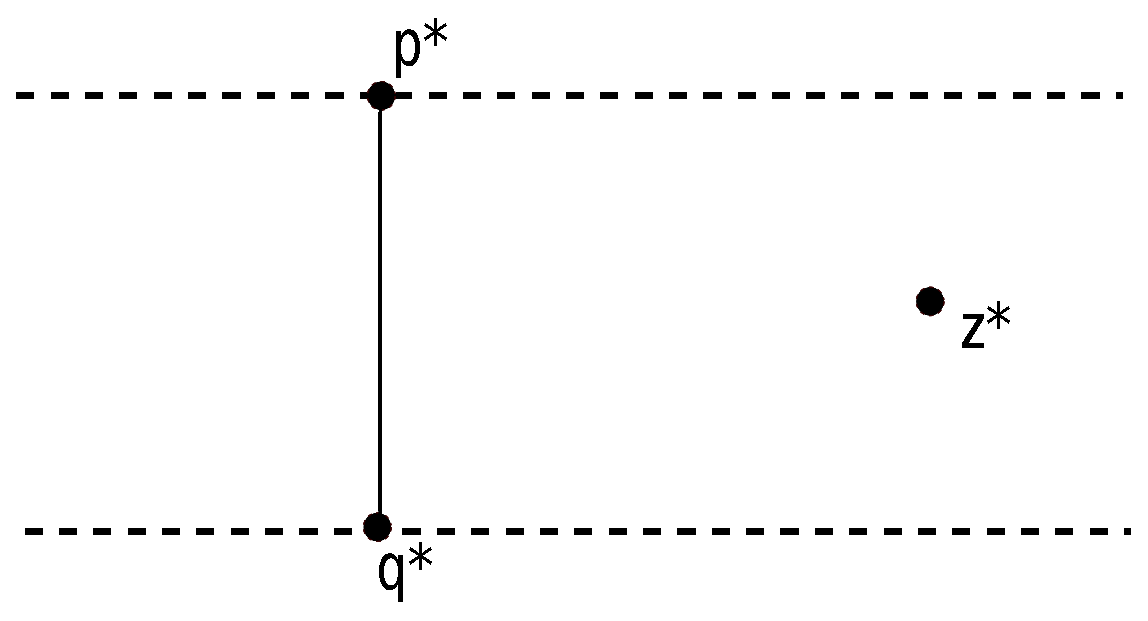
\includegraphics{figures/eps/pqz.eps}}}\hspace{-3em}%
\caption[\textbf{Geometry of GA:  $\bm{p}^\ast$, $\bm{q}^\ast$ and $\bm{z}^\ast$}]
{\textbf{Geometry of GA:  $\bm{p}^\ast$, $\bm{q}^\ast$ and $\bm{z}^\ast$}}
\label{pqz}
\end{center}
\end{figure}

Our tests show $\bm{z}^\ast$ is between $\bm{p}^\ast$ and $\bm{q}^\ast$ 
and also equidistant from $\bm{p}^\ast$ and $\bm{q}^\ast$ in both haploid and diploid case. 
We also ran tests for population points. In haploid case, 
both infinite and haploid populations were between $\bm{p}^\ast$ and $\bm{q}^\ast$. 
In diploid case, infinite population was between $\bm{p}^\ast$ and $\bm{q}^\ast$ but finite population was not. 
These are few geometric properties of GA uncovered by our simulations. 
Perhaps there are more geometric properties and details that can be discovered through simulations of evolutionary system.
That could be our future investigation.

In this research, we consider only uniform fitness for selection.  
In the future, we plan to extend our work by accomodating different fitness functions in our model and investigate 
the influence of that change upon the results obtained in the absence of selective pressure.



